\subsection*{Antaŭparolo}

Tiu ĉi libreto enhavas melodiojn por kordinstrumenteto nomiĝanta «Ukulelo» (tio nomo, {\fontspec{Gentium}ʻ}ukulele, venas el la havaja lingvo kaj signifas «saltanta pulo»). La libreto celas al komencantoj, kaj tio videblas per kelkaj manieroj:

\begin{compactitem}
	\item בחירה במנגינות מוכרות, חלקן שירים ידועים בעברית. לא כולן בהכרח „הלחם והטחינה” של כולם, אבל אני די בטוח שלפחות את חלקן תזהו.
	\item החוברת כוללת את הקו המלודי של המנגינות, ולא ליווי באקורדים, שהם לא שקופים להבנה.
	\item עיבדתי את המנגינות כך שבכל רגע נתון פורטים רק על מיתר אחד (מונופוניה). אחרי שתתאמנו על כל המנגינות שבחוברת תהיו מוכנים לגמרי לנגן כמה קולות (פוליפוניה).
	\item עריכה מסיבית של הקטעים הקלאסיים: קיצור, פישוט והשׂאה (טרנספוזיציה).
	\item אופן ההצגה: בנוסף לסימון תווים בשיטה המערבית הרגילה לפי גובה הצליל, מצורפת טבלטורה. הטבלטורה מסמנת בדיוק על איזה סריג ללחוץ ועל איזה מיתר לפרוט (ולכן היא מתאימה לאוקוללה לפי הכיוון הרגיל בלבד, ולא לכלים אחרים). באופן כזה, כשהתווים הרגילים והטבלטורה נמצאים אחד מעל השני, מי שיודעים לקרוא תווים יכולים לקרוא גם אותם (ולנגן לפיהם בכלי־נגינה אחרים), וכולם יכולים לנגן לפי הטבלטורה.
\end{compactitem}
רמת הקושי של הנעימות לא אחידה, ובמתכוון הן מעורבבות מבחינה זו ומסודרות לפי סדר אלפביתי. אני מציע להתחיל משירים מוכרים ופשוטים יותר, ולסיים בבורה של באך ובמנגינה של האחים סופר מריו, שהן היצירות המורכבות ביותר לביצוע בחוברת.



\subsection*{Agordo}

\begin{wrapfigure}[5]{r}{3.5cm}\vspace{-2\baselineskip}
	\begin{lilypond}
		theChords = \chordmode {g4 c e a}
		music = {g'4\4 c' e' a'}
		<<
		\new ChordNames { \theChords }
		\new Staff \with { \omit StringNumber \hide Staff.TimeSignature}
		\music
		\new TabStaff \with {stringTunings = \stringTuning <g' c' e' a'>}
		\music
		>>
	\end{lilypond}
\end{wrapfigure}
Ukulelo havas kvar kordojn, kiuj agordas iom strange: ne laŭ la tonalto, kiel la plimulto de kordinstrumentoj, sed laŭ alia ordo~— la unua kordo\footnote{La pli proksima al la kapo kiam vi ludas la Ukulelon; la pli malalta en la tabulaturo.} agordas, en la kutima agordo, kiel \emph{sol} (G), la sekva kiel \emph{do} (C) an la sama oktavo, sekvita per \emph{mi} (E) kaj \emph{la} (A). Tamaniere:

La pli facila maniero por agordi la ukulelo estas kun elektronika agordilo, kiun oni ***: . Estas grava, ke vi prenos universalan (kromatan) agordilon, ne unu, kiu celas nur al gitaro.
הדרך הכי קלה לכוון את האוקוללה היא בעזרת מכשיר כיוון אלקטרוני שמצמידים בתופסן לקצה הכלי: הוא חש את הרעידות ומתרגם אותן לסימון של גובה הצליל. חשוב שתשיגו מכוון שלא מותאם לגיטרה בלבד אלא כזה שהוא כללי (כרומטי).



\subsection*{Kiel oni legas tabulaturon?}

La ukulelo havas kvar kordojn, ĉu ne? Do, la tabulaturo havas kvar linoj, kiuj representas la kvar kordojn (kvazaŭ ĝi estas ukulelo, kiu restas kun ĝia kapo maldekstre). Dekstruloj plektras kun la dekstra mano kaj ***as kun la maldesktra.

נכון שלאוקוללה יש ארבעה מיתרים? אז לטבלטורה יש ארבע שורות, שמייצגות את ארבעת המיתרים (כאילו היא אוקוללה שמונח עם הראש בצד שמאל). ימניים פורטים עם יד ימין ולוחצים בין הסריגים ביד שמאל.

Oni legas tabulaturon de maldekstre, kiel la kutiman muzikan notacion. ***: «0» signifas plektri la decan malferman kordon, sen preni neniu*** freton; «1» signifas plektri preni la unua freton kaj plektri la decan kordon; «2» signifas la dua, k.t.p. Kutime ukuleloj havas signojn por indiki la fretoj facile (ekzemple, la 5a, 7a, 10a kaj la 12a). Jen tri ekzemploj por ludi tri aliaj tonoj:

\vspace{\baselineskip}
\begin{minipage}{4cm}
	\centering
	\includegraphics[width=3cm]{../plano-C3.eps}\\
	\begin{lilypond}
		music = {dis' \bar "|"}
		<<
		\new Staff \with { \omit StringNumber \hide Staff.TimeSignature}
		\music
		\new TabStaff \with {stringTunings = \stringTuning <g' c' e' a'>}
		\music
		>>
	\end{lilypond}
\end{minipage}\hfill
\begin{minipage}{4cm}
	\centering
	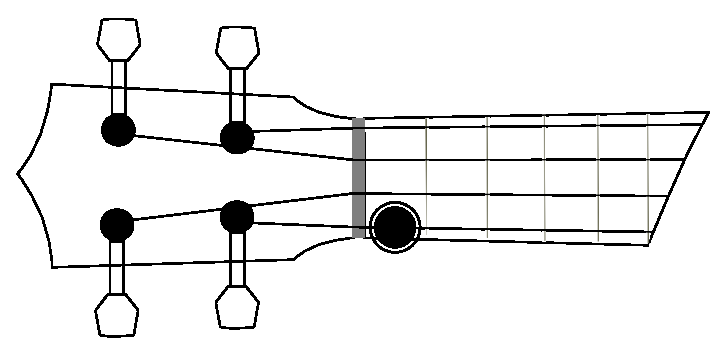
\includegraphics[width=3cm]{../plano-G1.eps}\\
	\begin{lilypond}
		music = {gis'\4 \bar "|"}
		<<
		\new Staff \with { \omit StringNumber \hide Staff.TimeSignature}
		\music
		\new TabStaff \with {stringTunings = \stringTuning <g' c' e' a'>}
		\music
		>>
	\end{lilypond}
\end{minipage}\hfill
\begin{minipage}{4cm}
	\centering
	\includegraphics[width=3cm]{../plano-A2.eps}\\
	\begin{lilypond}
		music = {b' \bar "|"}
		<<
		\new Staff \with { \omit StringNumber \hide Staff.TimeSignature}
		\music
		\new TabStaff \with {stringTunings = \stringTuning <g' c' e' a'>}
		\music
		>>
	\end{lilypond}
\end{minipage}
\vspace{\baselineskip}

La daŭroj de la tonoj estas indikitaj tie ĉi nur sur la tonalta notacio, normale: \symbolglyph{𝅝} signifas plenan daŭron (\L{1}), \symbolglyph{𝅗𝅥} signifas duona (\L{½}), \symbolglyph{𝅘𝅥} signifas kvarona (\L{¼}), kaj \symbolglyph{𝅘𝅥𝅮} aŭ \symbolglyph{♫} signifas okona (\L{⅛}); la egalvaloroj de la paŭzoj estas \symbolglyph{𝄻}, \symbolglyph{𝄼}, \symbolglyph{𝄽} ו־\symbolglyph{𝄾}, respektive.

Ĉu vi volas certigi, ke vi bone komprenas? Jen la komenco de «Hanseto la Malgranda» (\emph{Hänschen klein}\footnote{\url{https://commons.wikimedia.org/wiki/File:Picking_Haenschen_klein_einfach.mid}}). Provu ludi tion:

\begin{center}
	\begin{lilypond}
		music = {
			\time 4/4
			\transpose c c' {
				<g\4>4 <e\2>4 <e\2>2
				<f\2>4 <d\3>4 <d\3>2
				<c\3>4 <d\3>4 <e\2>4 <f\2>4
				<g\4>4 <g\4>4 <g\4>2
			}
		}
		<<
		\new Staff \with { \omit StringNumber \hide Staff.TimeSignature}
		\music
		\new TabStaff \with {stringTunings = \stringTuning <g' c' e' a'>}
		\music
		>>
	\end{lilypond}
\end{center}

Ripetoj estas indikitaj per \symbolglyph{𝄆} kaj \symbolglyph{𝄇}. Kiam la du ripetoj estas malsama, la malsamaj finaĵoj estas indikitaj per numeritaj \symbolglyph{⌜} signoj sur ili.



\subsection*{Informo kaj kontaktimformo}

\begin{wrapfigure}[4]{r}{1.75cm}\vspace{-\baselineskip}\includegraphics[width=1.5cm]{../retejo.png}\end{wrapfigure}
	La retejo de la libreto estas \url{http://xpr.digitalwords.net/ukulele} (QR-kodo estas dekstre). Ĉe la retejo estas plia informo kaj ligiloj, krome***
האתר של החוברת הוא \url{http://xpr.digitalwords.net/ukulele} (קוד \L{QR} בצד שמאל). באתר מידע נוסף וקישורים, כמו גם כל קבצי המקור של החוברת וקובץ מוכן להדפסה (אם תרצו ליצור עותק נוסף או לקרוא במחשב). את הטבלטורות הכנתי בעזרת התוכנה החופשית \L{TuxGuitar}\footnote{זו תוכנה פשוטה, מדי, שנעדרת כמה תכונות בסיסיות; כך, לדוגמה, בחלק מהמקומות מופיע בתווים „סול במול” במקום „פה דיאז”, ולא מצאתי דרך לשנות את זה. גם הסימון של ${1}\over{16}$ יחידים לא ברור מספיק, ואין תמיכה בתיבות שאינן שלמות.}; היא זמינה להורדה בכתובת \url{http://tuxguitar.com.ar}. אם תפתחו את קבצי המקור של המנגינות (סיומת \texttt{.tg}) בתוכנה הזאת תוכלו לשמוע אותן כשבזמן אמת מסומן המקום המתאים בטבלטורה ובתווים, כמו גם אופן הנגינה על ציור סכימטי של אוקוללה.

Tiu ĉi libreto estas libera (publikaĵo): vi povas kopii, modifi, disdoni kaj uzi ĝin ielajn vi volas.

Pri ia ajn afero ne hezitu kontakti min per retpoŝto (\url{ukulele@digitalwords.net}) aŭ per telefono (972-2-6419913). Prencipe, mi ĝojus aŭdi ***
בכל עניין, אל תהססו לפנות אלי בדואל (\url{ukulele@digitalwords.net}) או בטלפון (02-6419913). בפרט, אשמח לשמוע כל מה יש לכם להגיד על החוברת, ולקבל הצעות, שיפורים ותיקונים\footnote{חלק מהמנגינות כתבתי משמיעה, ויש מה לשפר ולדייק בהן.}.

\vspace{\baselineskip}
~\hfill
\begin{minipage}{3cm}
	Júda Ronén\\
	Jerusalemo 2014\\
\end{minipage}
